\documentclass[12pt]{article}
\usepackage[utf8]{inputenc}
\usepackage{amsmath}
\usepackage{amsfonts}
\usepackage{amssymb}
\usepackage{empheq}
\usepackage{tikz}
\usetikzlibrary{automata, positioning, shapes}
\addtolength{\topmargin}{-0.875in}
\addtolength{\textheight}{1.75in}

\title{Regarding Positive Even Zeta Values}
\author{Ethan Jensen}
\date{October 12th, 2019}

\begin{document}
	\maketitle
	\tikzset{
		node distance=3cm, % specifies the minimum distance between two nodes. Change if necessary.
		initial text=$ $, % sets the text that appears on the start arrow
	}
\definecolor{mycolor1}{RGB}{230,230,230}
\definecolor{mycolor2}{RGB}{210,210,210}
\definecolor{mycolor3}{RGB}{190,190,190}
\section[20pt]{Analyzing Positive Even Zeta Values}
The Riemann Zeta function is a complex-valued function that accepts a complex number as an argument. This paper will focus entirely on the Zeta function evaluated at positive even integer values. Positive even Zeta values have an exact form in terms of \(\pi\) and can be calculated recursively several ways. This paper will explain two different ways of calculating said values. \newline \newline
The Riemann Zeta and Dirichlet Eta functions are defined as follows
\[\zeta(s)=\sum_{n=1}^{\infty}\frac{1}{n^s},\ \  \eta(s)=\sum_{n=1}^{\infty}\frac{(-1)^{n-1}}{n^s}\]
Trivially, we can show that \[\eta(s)=(1-2^{1-s})\zeta(s)\]
\textbf{Proof.}
\[\eta(s) = \frac{1}{1^s} - \frac{1}{2^s} + \frac{1}{3^s} - \frac{1}{4^s} + \frac{1}{5^s} - \frac{1}{6^s}...\]
\[\eta(s) = \frac{1}{1^s} + \frac{1}{2^s} + \frac{1}{3^s} + \frac{1}{4^s} + \frac{1}{5^s}...-2\left[\frac{1}{2^s} + \frac{1}{4^s} + \frac{1}{6^s}...\right]\]
\[\eta(s) = \frac{1}{1^s} + \frac{1}{2^s} + \frac{1}{3^s} + \frac{1}{4^s} + \frac{1}{5^s}...-\frac{2}{2^s}\left[\frac{1}{1^s} + \frac{1}{2^s} + \frac{1}{3^s}...\right]\]
\[\eta(s)=\zeta(s)-\frac{2}{2^s}\zeta(s)=(1-2^{1-s})\zeta(s)\]
\(\blacksquare\) \newline
\newpage
\section{Infinite Polynomials}
\textbf{Theorem 1.1.}
\[1+\frac{\pi^2x^2}{3!}+\frac{\pi^4x^4}{5!}+\frac{\pi^6x^6}{7!}...=\left(1+\frac{x^2}{1^2}\right)\left(1+\frac{x^2}{2^2}\right)\left(1+\frac{x^2}{3^2}\right)...\]
\textbf{Proof.} \newline
We start by comparing the MacLaurin series of \(\sinh(x)\) with the product expansion of \(\sinh(x)\). Note that the roots of \(\sinh(x)\) are \(k\pi i\) by Euler's formula.
\[\sinh(x)=\frac{x}{1!} + \frac{x^3}{3!} + \frac{x^5}{5!} + \frac{x^7}{7!}... =x\left(1+\frac{x}{i\pi}\right)\left(1-\frac{x}{i\pi}\right)\left(1+\frac{x}{2i\pi}\right)\left(1-\frac{x}{2i\pi}\right)\left(1+\frac{x}{3i\pi}\right)...\]
\[\frac{\sinh(x)}{x}=\frac{1}{1!} + \frac{x^2}{3!} + \frac{x^4}{5!} + \frac{x^6}{7!}...=\left(1+\frac{x^2}{\pi^2}\right)\left(1+\frac{x^2}{2^2\pi^2}\right)\left(1+\frac{x^2}{3^2\pi^2}\right)...\]
\[\frac{\sinh(\pi x)}{x}=1+\frac{\pi^2x^2}{3!}+\frac{\pi^4x^4}{5!}+\frac{\pi^6x^6}{7!}...=\left(1+\frac{x^2}{1^2}\right)\left(1+\frac{x^2}{2^2}\right)\left(1+\frac{x^2}{3^2}\right)...\]
\(\blacksquare\)
\newline
When multiplying a product, to calculate the coefficient on a polynomial of the nth degree, all term combinations resulting in the nth degree of each factor must be determined and subsequently summed. \newline
\newline
For the product expansion, the only term combinations resulting in degree 2 are when we select one \(x^2\) term from one factor at a time and select a 1 from the other factors. Comparing this to the right hand side we have
\[\frac{\pi^2}{3!}=\frac{1}{1^2}+\frac{1}{2^2}+\frac{1}{3^2}+\frac{1}{4^2}...\]
Thus, using our definition of the Zeta function we have
\[\zeta(2)=\frac{\pi^2}{6}.\]
This result is incredible in and of itself, but Theorem 1.1 is the basis for computing all positive even Zeta values.
\newline
\newline
To find subsequent even Zeta values, coefficients of higher degree must be calculated for the infinite product and compared to the coefficient on the corresponding term in the infinite sum. \newline
\newline
For example, Theorem 1.1 implies that
\[\sum_i\sum_{j<i}\frac{1}{i^2}\frac{1}{j^2}=\frac{\pi^4}{5!}\]
\newpage
\section{Motivation for Using Disjoint Partitions}
It is often useful to use geometry to aid in understanding a concept in smaller dimensions, and then using algebra to generalize to higher dimensions. \newline
Consider the following infinitely big "Addition Square"
\begin{figure}[ht]
	\centering % centers the figure
	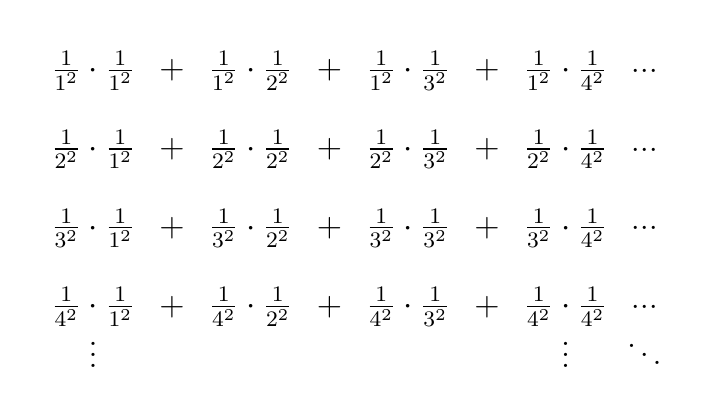
\begin{tikzpicture}[inner sep=3mm]
	\node[] (L1) at (0,0) {\large $\frac{1}{4^2}\cdot\frac{1}{1^2}$};
	\node[] (L2) at (1,0) {\large $+$};
	\node[] (L1) at (2,0) {\large $\frac{1}{4^2}\cdot\frac{1}{2^2}$};
	\node[] (L2) at (3,0) {\large $+$};
	\node[] (L1) at (4,0) {\large $\frac{1}{4^2}\cdot\frac{1}{3^2}$};
	\node[] (L2) at (5,0) {\large $+$};
	\node[] (L1) at (6,0) {\large $\frac{1}{4^2}\cdot\frac{1}{4^2}$};
	\node[] (L2) at (7,0) {\large $...$};

	\node[] (L1) at (0,1) {\large $\frac{1}{3^2}\cdot\frac{1}{1^2}$};
	\node[] (L2) at (1,1) {\large $+$};
	\node[] (L1) at (2,1) {\large $\frac{1}{3^2}\cdot\frac{1}{2^2}$};
	\node[] (L2) at (3,1) {\large $+$};
	\node[] (L1) at (4,1) {\large $\frac{1}{3^2}\cdot\frac{1}{3^2}$};
	\node[] (L2) at (5,1) {\large $+$};
	\node[] (L1) at (6,1) {\large $\frac{1}{3^2}\cdot\frac{1}{4^2}$};
	\node[] (L2) at (7,1) {\large $...$};

	\node[] (L1) at (0,2) {\large $\frac{1}{2^2}\cdot\frac{1}{1^2}$};
	\node[] (L2) at (1,2) {\large $+$};
	\node[] (L1) at (2,2) {\large $\frac{1}{2^2}\cdot\frac{1}{2^2}$};
	\node[] (L2) at (3,2) {\large $+$};
	\node[] (L1) at (4,2) {\large $\frac{1}{2^2}\cdot\frac{1}{3^2}$};
	\node[] (L2) at (5,2) {\large $+$};
	\node[] (L1) at (6,2) {\large $\frac{1}{2^2}\cdot\frac{1}{4^2}$};
	\node[] (L2) at (7,2) {\large $...$};

	\node[] (L1) at (0,3) {\large $\frac{1}{1^2}\cdot\frac{1}{1^2}$};
	\node[] (L2) at (1,3) {\large $+$};
	\node[] (L1) at (2,3) {\large $\frac{1}{1^2}\cdot\frac{1}{2^2}$};
	\node[] (L2) at (3,3) {\large $+$};
	\node[] (L1) at (4,3) {\large $\frac{1}{1^2}\cdot\frac{1}{3^2}$};
	\node[] (L2) at (5,3) {\large $+$};
	\node[] (L1) at (6,3) {\large $\frac{1}{1^2}\cdot\frac{1}{4^2}$};
	\node[] (L2) at (7,3) {\large $...$};

	\node[] (L3) at (0,-0.5) {\large $\vdots$};
	\node[] (L3) at (6,-0.5) {\large $\vdots$};
	\node[] (L3) at (7,-0.5) {\large $\ddots$};
	\end{tikzpicture}
	\caption{Addition Square}
\end{figure}
\newline
By the distributive property, the "Addition Square" can be written as \[\left(\frac{1}{1^2}+\frac{1}{2^2}+\frac{1}{3^2}...\right)^2=\zeta(2)^2=\frac{\pi^4}{36}\]
\newline
The Addition Square can also be split up into three smaller summations.
\begin{figure}[ht]
	\centering % centers the figure
	\begin{tikzpicture}[inner sep=3mm]
	\filldraw [fill=mycolor3] (-0.7,3.5) rectangle (0.7,2.5);
	\filldraw [fill=mycolor1] (1.3,3.5) rectangle (2.7,2.5);
	\filldraw [fill=mycolor1] (3.3,3.5) rectangle (4.7,2.5);
	\filldraw [fill=mycolor1] (5.3,3.5) rectangle (6.7,2.5);

	\filldraw [fill=mycolor1] (-0.7,2.5) rectangle (0.7,1.5);
	\filldraw [fill=mycolor3] (1.3,2.5) rectangle (2.7,1.5);
	\filldraw [fill=mycolor1] (3.3,2.5) rectangle (4.7,1.5);
	\filldraw [fill=mycolor1] (5.3,2.5) rectangle (6.7,1.5);

	\filldraw [fill=mycolor1] (-0.7,1.5) rectangle (0.7,0.5);
	\filldraw [fill=mycolor1] (1.3,1.5) rectangle (2.7,0.5);
	\filldraw [fill=mycolor3] (3.3,1.5) rectangle (4.7,0.5);
	\filldraw [fill=mycolor1] (5.3,1.5) rectangle (6.7,0.5);

	\filldraw [fill=mycolor1] (-0.7,0.5) rectangle (0.7,-0.5);
	\filldraw [fill=mycolor1] (1.3,0.5) rectangle (2.7,-0.5);
	\filldraw [fill=mycolor1] (3.3,0.5) rectangle (4.7,-0.5);
	\filldraw [fill=mycolor3] (5.3,0.5) rectangle (6.7,-0.5);
	\node[] (L1) at (0,0) {\large $\frac{1}{4^2}\cdot\frac{1}{1^2}$};
	\node[] (L2) at (1,0) {\large $+$};
	\node[] (L1) at (2,0) {\large $\frac{1}{4^2}\cdot\frac{1}{2^2}$};
	\node[] (L2) at (3,0) {\large $+$};
	\node[] (L1) at (4,0) {\large $\frac{1}{4^2}\cdot\frac{1}{3^2}$};
	\node[] (L2) at (5,0) {\large $+$};
	\node[] (L1) at (6,0) {\large $\frac{1}{4^2}\cdot\frac{1}{4^2}$};
	\node[] (L2) at (7,0) {\large $...$};

	\node[] (L1) at (0,1) {\large $\frac{1}{3^2}\cdot\frac{1}{1^2}$};
	\node[] (L2) at (1,1) {\large $+$};
	\node[] (L1) at (2,1) {\large $\frac{1}{3^2}\cdot\frac{1}{2^2}$};
	\node[] (L2) at (3,1) {\large $+$};
	\node[] (L1) at (4,1) {\large $\frac{1}{3^2}\cdot\frac{1}{3^2}$};
	\node[] (L2) at (5,1) {\large $+$};
	\node[] (L1) at (6,1) {\large $\frac{1}{3^2}\cdot\frac{1}{4^2}$};
	\node[] (L2) at (7,1) {\large $...$};

	\node[] (L1) at (0,2) {\large $\frac{1}{2^2}\cdot\frac{1}{1^2}$};
	\node[] (L2) at (1,2) {\large $+$};
	\node[] (L1) at (2,2) {\large $\frac{1}{2^2}\cdot\frac{1}{2^2}$};
	\node[] (L2) at (3,2) {\large $+$};
	\node[] (L1) at (4,2) {\large $\frac{1}{2^2}\cdot\frac{1}{3^2}$};
	\node[] (L2) at (5,2) {\large $+$};
	\node[] (L1) at (6,2) {\large $\frac{1}{2^2}\cdot\frac{1}{4^2}$};
	\node[] (L2) at (7,2) {\large $...$};

	\node[] (L1) at (0,3) {\large $\frac{1}{1^2}\cdot\frac{1}{1^2}$};
	\node[] (L2) at (1,3) {\large $+$};
	\node[] (L1) at (2,3) {\large $\frac{1}{1^2}\cdot\frac{1}{2^2}$};
	\node[] (L2) at (3,3) {\large $+$};
	\node[] (L1) at (4,3) {\large $\frac{1}{1^2}\cdot\frac{1}{3^2}$};
	\node[] (L2) at (5,3) {\large $+$};
	\node[] (L1) at (6,3) {\large $\frac{1}{1^2}\cdot\frac{1}{4^2}$};
	\node[] (L2) at (7,3) {\large $...$};

	\node[] (L3) at (0,-0.5) {\large $\vdots$};
	\node[] (L3) at (6,-0.5) {\large $\vdots$};
	\node[] (L3) at (7,-0.5) {\large $\ddots$};
	\end{tikzpicture}
	\caption{Addition Partition}
\end{figure}
\newline
The Diagonal Summation is equal to \(\zeta(4)\).
As for the Triangle Summations, we make use of Theorem 1.1.
\[1+\frac{\pi^2x^2}{3!}+\frac{\pi^4x^4}{5!}+\frac{\pi^6x^6}{7!}...=\left(1+\frac{x^2}{1^2}\right)\left(1+\frac{x^2}{2^2}\right)\left(1+\frac{x^2}{3^2}\right)...\]
Each Triangle Summation is the term sum of all term combinations of two factors in the infinite product and thus equal to the corresponding series expansion coefficient \(\frac{\pi^4}{5!}\). Thus,
\[\frac{\pi^4}{36}=2\frac{\pi^4}{120}+\zeta(4)\implies\zeta(4)=\frac{\pi^4}{90}\]
\newpage
\section{Condition Codes for Disjoint Partitions}
One useful way of constructing a disjoint partition of a multidimensional set is to separate sets by grouping. More specifically, separating sets based on the sizes of groups in which elements in particular dimensions are equal to each other. For the purposes of this paper, the Universal set for each element \(x_1,x_2,...\) will be \(\mathbb{Z}^+\).\newline \newline
This partitioning means that sets can be given a unique condition code that describes the amount of groups of a certain size contained in said set. \newline
\newline
For example, the set \(\{(x_1,x_2,x_3):x_1=x_2\neq x_3\}\)
can be given the condition code (1,2) signifying exactly 1 group of size 1 (\(x_3\)), and one group of size 2 (\(x_1=x_2\)). \newline \newline
We can then describe our universal set \({\mathbb{Z}^+}^n\) as the union of all the subsets where the condition codes are of the form \((a_1,a_2,a_3...a_k)\) where \(a_1+a_2+a_3...+a_k=n\). \newline \newline
\textbf{Example 1.1} \newline
Express \({\mathbb{Z}^+}^4\) as a disjoint partition of sets.
\newline
\[{\mathbb{Z}^+}^4=A_1\cup A_2\cup A_3\cup A_4\cup A_5\]
where the condition codes for the sets \(A_1\) through \(A_5\) are as follows.
\[A_1:(1,1,1,1);\ \ A_2:(1,1,2);\ \ A_3:(1,3);\ \ A_4:(2,2);\ \ A_5:(4)\]
In set-builder notation, each of the sets \(A_1\) through \(A_5\) are themselves a union of smaller subsets with similar equality and inequality conditions. For example \(A_3\) is the union of the four following smaller subsets which will be referred to as \textbf{spicy subsets}.
\[A_3=\{(x_1,x_2,x_3,x_4):x_1=x_2=x_3\neq x_4\}\cup\{(x_1,x_2,x_3,x_4):x_1=x_2=x_4\neq x_3\}\]\[\cup\{(x_1,x_2,x_3,x_4):x_1=x_3=x_4\neq x_2\}\cup\{(x_1,x_2,x_3,x_4):x_2=x_3=x_4\neq x_1\}\]
\(\blacksquare\) \newline \newline
This partition is complete because it ranges over the full possibilities for the condition codes. It is disjoint because the conditions of each set are unique. \newline \newline
The exact number of spicy subsets \(a\) for each \(A_1\) through \(A_5\) is very important and can be determined using an analogy called "Blocks and Holes" which will be discussed later.

\newpage
\section{The D Function}
\textbf{Definition 1.1.}
\[D(a_1,a_2,a_3...)=\sum_{a\in A}\frac{1}{(x_1)^2}\frac{1}{(x_2)^2}...\frac{1}{(x_n)^2},\ A \textup{ has condition code } (a_1,a_2,a_3...)\]
where \(a\) is a previously mentioned spicy subset of \(A\). \newline
For example, \[D(1,2)=\frac{1}{1^2}\frac{1}{2^4}+\frac{1}{1^2}\frac{1}{3^4}+\frac{1}{1^2}\frac{1}{4^4}+\frac{1}{2^2}\frac{1}{1^4}+\frac{1}{2^2}\frac{1}{2^4}+\frac{1}{2^2}\frac{1}{3^4}+\frac{1}{2^2}\frac{1}{4^4}+\frac{1}{3^2}\frac{1}{1^4}...\]
\newline
\textbf{Theorem 1.2.}
\(D(n)=\zeta(2n), n\in\mathbb{Z}^+\) \newline
\textbf{Proof.} \newline
By Definition 1.1
\[D(n)=\sum_{a\in A}\frac{1}{(x_1)^{2}}\frac{1}{(x_2)^{2}}...\frac{1}{(x_3)^{2}},\ \ A={\mathbb{Z}^+}^n\]
\[\textup{by the transitive property of equality } \exists!a\in A \textup{ which implies that } a = {\mathbb{Z}^+}^n\]
\[D(n)=\sum_{k=1}^{\infty}\frac{1}{k^{2n}}=\zeta(2n)\]
\(\blacksquare\) \newline
\textbf{Definition 1.2.}
\[D^{k}(a_1,a_2,...a_n)=\left(D(a_1,a_2,...a_n)\right)^k\]
\[D_k(a_1)=D(a_1,a_1,a_1...a_1) \textup{, which has k arguments}\]
For example,
\[D^3(2)=D(2)D(2)D(2)\]
\[D_3(1)=D(1,1,1)\]
\textbf{Theorem 1.3.} \(D_n(1)= \frac{\pi^{2n}}{(2n+1)!}\) \newline
\textbf{Proof.} \newline
By Theorem 1.1 The product form must match the series form of \(\frac{\sinh(x)}{x}\). It's coefficient is calculated by the sum of n term combinations of coefficients of \(x^{2n}\). Thus,
\[\frac{1}{(2n+1)!}=\sum_a\frac{1}{\pi^{2}(x_1)^2}\frac{1}{\pi^{2}(x_2)^2}...\frac{1}{\pi^{2}(x_n)^2},\ a=\{(x_1,x_2,...x_n):x_1< x_2...< x_n\} \]
\[\frac{\pi^{2n}}{(2n+1)!}=\sum_{a\in A}\frac{1}{(x_1)^{2}}\frac{1}{(x_2)^{2}}...\frac{1}{(x_n)^{2}},\ \ A=(1,1,1,1,1...) \textup{ with n terms.}\]
\[\frac{\pi^{2n}}{(2n+1)!}=D_n(1)\]
\(\blacksquare\)
\newpage
\section{Algebra with the D function}
Via \textbf{Theorem 1.2} and \textbf{Theorem 1.3} we have a connection between the Zeta function and \(\pi\). To do the algebra, we need one final Theorem. \newline
\textbf{Theorem 1.4} \newline
\(D(C)\) can always be expressed as a sum \(p_1D(C_1)+p_2D(C_2)+p_3D(C_3)...+p_kD(C_k)\), where \(p_i\) is the number of spicy subsets for the set \(A_i\) with the corresponding condition code \(C_i\). \newline
\textbf{Example 1.2} \newline
Calculate \(\zeta(6)\), where \(\zeta(2) = \frac{\pi^2}{6},\ \zeta(4)=\frac{\pi^4}{90}\) \newline
By Theorem 1.4 we have the equations
\begin{equation}
D(1)(1)(1)=6D(1,1,1)+3D(1,2)+D(3)
\end{equation}
\begin{equation}
D(1)(2) = D(1,2) + D(3)
\end{equation}
From (2)
\begin{equation}
D(1,2) = D(1)(2) - D(3)
\end{equation}
Substituting (3) into (1)
\begin{equation}
D(1)(1)(1) = 6D(1,1,1) + 3D(1)(2) - 2D(3)
\end{equation}
By Theorem 1.2 and 1.3
\begin{equation}
\zeta(2)\zeta(2)\zeta(2) = 6\frac{\pi^6}{7!} + 3\zeta(2)\zeta(4) - 2\zeta(6)
\end{equation}
Plugging in values for \(\zeta(2)\) and \(\zeta(4)\) we have
\begin{equation}
\left(\frac{\pi^2}{6}\right)^3 = 6\frac{\pi^6}{7!} + 3\left(\frac{\pi^2}{6}\right)\left(\frac{\pi^4}{90}\right) - 2\zeta(6)
\end{equation}
Finally, we solve for \(\zeta(6)\). \newline
\boxed{\zeta(6)=\frac{\pi^6}{945}} \newline \newline
\(\blacksquare\) \newline
In equation 1, the coefficients 6,3, and 1, can be calculated by enumeration.
\begin{figure}[ht]
	\centering % centers the figure
	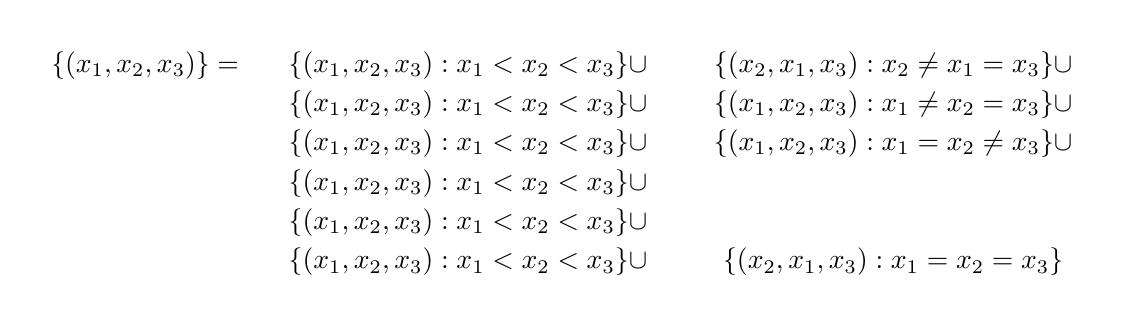
\begin{tikzpicture}[inner sep=3mm]
	\node[] (S1) at (0,2.5) {$\{(x_1,x_2,x_3)\}=$};

	\node[] (S2) at (4.1,0) {$\{(x_1,x_2,x_3):x_1<x_2<x_3\}\cup$};
	\node[] (S2) at (4.1,0.5) {$\{(x_1,x_2,x_3):x_1<x_2<x_3\}\cup$};
	\node[] (S2) at (4.1,1) {$\{(x_1,x_2,x_3):x_1<x_2<x_3\}\cup$};
	\node[] (S2) at (4.1,1.5) {$\{(x_1,x_2,x_3):x_1<x_2<x_3\}\cup$};
	\node[] (S2) at (4.1,2) {$\{(x_1,x_2,x_3):x_1<x_2<x_3\}\cup$};
	\node[] (S2) at (4.1,2.5) {$\{(x_1,x_2,x_3):x_1<x_2<x_3\}\cup$};

	\node[] (S2) at (9.5,0) {$\{(x_2,x_1,x_3):x_1=x_2=x_3\}$};

	\node[] (S2) at (9.5,1.5) {$\{(x_1,x_2,x_3):x_1=x_2\neq x_3\}\cup$};
	\node[] (S2) at (9.5,2) {$\{(x_1,x_2,x_3):x_1\neq x_2=x_3\}\cup$};
	\node[] (S2) at (9.5,2.5) {$\{(x_2,x_1,x_3):x_2\neq x_1=x_3\}\cup$};
	\end{tikzpicture}
	\caption{Spicy Subset Enumeration}
\end{figure}


\newpage
\section{Blocks and Holes}
We can use an analogy to calculate the number of spicy subsets. \newline \newline
Consider the following scenario. The scenario consists of a collection of labeled blocks of varying sizes and a collection of labeled holes of varying sizes. The goal is to count the number of ways of distributing the blocks into the holes perfectly.
\begin{itemize}
\item All blocks and holes are rectangles 1 unit wide. Their lengths are a whole number of units.
\item The total area of the blocks equals the total area of the holes.
\item The different ordering of blocks in a hole does not count as a separate arrangement.
\end{itemize}
\textbf{Example 1.3} \newline
Determine the number of ways of distributing the collection of blocks [1,1,2] into the holes [1,3].
\begin{figure}[ht]
	\centering % centers the figure
	\begin{tikzpicture}[inner sep=3mm]
\node[draw,fill=mycolor1] (B1) at (0,0) {};
\node[draw,fill=mycolor1] (B2) at (1,0) {};
\node[draw,fill=mycolor1] (B3) at (2,0) {};
\node[draw,fill=mycolor1] (B4) at (2,0.6) {};
\node[] (L1) at (0,-0.6) {$B_1$};
\node[] (L1) at (1,-0.6) {$B_2$};
\node[] (L1) at (2,-0.6) {$B_3$};
\node[] (L1) at (1,1.8) {Blocks};
\node[] (L1) at (4.5,1.8) {Holes};
\node[] (L1) at (4,0) {$H_1$};
\node[] (L1) at (5,0) {$H_2$};
\node[draw,fill=mycolor2,dashed] (H1) at (4,-0.6) {};
\node[draw,fill=mycolor2,dashed] (H2) at (5,-0.6) {};
\node[draw,fill=mycolor2,dashed] (H3) at (5,-1.2) {};
\node[draw,fill=mycolor2,dashed] (H4) at (5,-1.8) {};
\end{tikzpicture}
	\caption{Blocks and Holes Scenario 1.1}
\end{figure}
\begin{figure}[ht]
	\centering % centers the figure
	\begin{tikzpicture}[inner sep=3mm]
	\node[draw,fill=mycolor1] (B1) at (0,0) {};
	\node[draw,fill=mycolor1] (B2) at (1.5,0) {};
	\filldraw[fill=mycolor1] (1.8,-0.3) rectangle (1.2,-1.5);
	\node[] (L1) at (0.6,0) {$B_1$};
	\node[] (L1) at (2.1,0) {$B_2$};
	\node[] (L1) at (2.1,-0.6) {$B_3$};
	\node[] (L1) at (1,1.8) {1};
	\node[] (L1) at (4.5,1.8) {2};

	\node[draw,fill=mycolor1] (B1) at (3.5,0) {};
	\node[draw,fill=mycolor1] (B2) at (5,0) {};
	\filldraw[fill=mycolor1] (5.3,-0.3) rectangle (4.7,-1.5);
	\node[] (L1) at (4.1,0) {$B_2$};
	\node[] (L1) at (5.6,0) {$B_1$};
	\node[] (L1) at (5.6,-0.6) {$B_3$};

	\end{tikzpicture}
	\caption{Blocks and Holes Solution 1.1}
\end{figure}
\newline
Thus, by enumeration, the number of arrangements of the Blocks [1,1,2] into the Holes [1,3] is 2.
\newpage
\section{Blocks and Holes cont.}
\textbf{Example 1.4}
Determine the number of ways of distributing the collection of Blocks[1,1,1] into the Holes [1,1,1].
\begin{figure}[ht]
	\centering % centers the figure
	\begin{tikzpicture}[inner sep=3mm]
	\node[draw,fill=mycolor1] (B1) at (0,0) {};
	\node[draw,fill=mycolor1] (B2) at (1,0) {};
	\node[draw,fill=mycolor1] (B3) at (2,0) {};
	\node[] (L1) at (0,-0.6) {$B_1$};
	\node[] (L1) at (1,-0.6) {$B_2$};
	\node[] (L1) at (2,-0.6) {$B_3$};
	\node[] (L1) at (1,1.8) {Blocks};
	\node[] (L1) at (4.5,1.8) {Holes};
	\node[] (L1) at (4,0) {$H_1$};
	\node[] (L1) at (5,0) {$H_2$};
	\node[] (L1) at (6,0) {$H_3$};
	\node[draw,fill=mycolor2,dashed] (H1) at (4,-0.6) {};
	\node[draw,fill=mycolor2,dashed] (H2) at (5,-0.6) {};
	\node[draw,fill=mycolor2,dashed] (H3) at (6,-0.6) {};
	\end{tikzpicture}
	\caption{Blocks and Holes Scenario 1.2}
\end{figure}
\begin{figure}[ht]
	\centering % centers the figure
	\begin{tikzpicture}[inner sep=3mm]
	\node[draw,fill=mycolor1] (B1) at (0,0) {};
	\node[draw,fill=mycolor1] (B2) at (1.5,0) {};
	\node[draw,fill=mycolor1] (B3) at (3,0) {};

	\node[] (L1) at (0.6,0) {$B_1$};
	\node[] (L1) at (2.1,0) {$B_2$};
	\node[] (L1) at (3.6,0) {$B_3$};
	\node[] (L1) at (1.5,0.9) {1};

	\node[draw,fill=mycolor1] (B1) at (5,0) {};
	\node[draw,fill=mycolor1] (B2) at (6.5,0) {};
	\node[draw,fill=mycolor1] (B3) at (8,0) {};

	\node[] (L1) at (5.6,0) {$B_1$};
	\node[] (L1) at (7.1,0) {$B_3$};
	\node[] (L1) at (8.6,0) {$B_2$};
	\node[] (L1) at (6.5,0.9) {2};

	\node[draw,fill=mycolor1] (B1) at (10,0) {};
	\node[draw,fill=mycolor1] (B2) at (11.5,0) {};
	\node[draw,fill=mycolor1] (B3) at (13,0) {};

	\node[] (L1) at (10.6,0) {$B_2$};
	\node[] (L1) at (12.1,0) {$B_1$};
	\node[] (L1) at (13.6,0) {$B_3$};
	\node[] (L1) at (11.5,0.9) {3};


	\node[draw,fill=mycolor1] (B1) at (0,-2) {};
	\node[draw,fill=mycolor1] (B2) at (1.5,-2) {};
	\node[draw,fill=mycolor1] (B3) at (3,-2) {};

	\node[] (L1) at (0.6,-2) {$B_2$};
	\node[] (L1) at (2.1,-2) {$B_3$};
	\node[] (L1) at (3.6,-2) {$B_1$};
	\node[] (L1) at (1.5,-1.1) {4};

	\node[draw,fill=mycolor1] (B1) at (5,-2) {};
	\node[draw,fill=mycolor1] (B2) at (6.5,-2) {};
	\node[draw,fill=mycolor1] (B3) at (8,-2) {};

	\node[] (L1) at (5.6,-2) {$B_3$};
	\node[] (L1) at (7.1,-2) {$B_1$};
	\node[] (L1) at (8.6,-2) {$B_2$};
	\node[] (L1) at (6.5,-1.1) {5};

	\node[draw,fill=mycolor1] (B1) at (10,-2) {};
	\node[draw,fill=mycolor1] (B2) at (11.5,-2) {};
	\node[draw,fill=mycolor1] (B3) at (13,-2) {};

	\node[] (L1) at (10.6,-2) {$B_3$};
	\node[] (L1) at (12.1,-2) {$B_2$};
	\node[] (L1) at (13.6,-2) {$B_1$};
	\node[] (L1) at (11.5,-1.1) {6};
	\end{tikzpicture}
	\caption{Blocks and Holes Solution 1.2}
\end{figure}
\newline
Thus, by enumeration, the number of Blocks[1,1,1] into the Holes[1,1,1] is 6. \newline \newline


\newpage
\section{Blocks and Holes cont.}
\textbf{Example 1.5} \newline
Determine the number of ways of distributing the collection of Blocks [1,1,1,2,3] into the Holes [1,3,4].
\begin{figure}[ht]
	\centering % centers the figure
	\begin{tikzpicture}[inner sep=3mm]
	\node[draw,fill=mycolor1] (B1) at (0,0) {};
	\node[draw,fill=mycolor1] (B2) at (1,0) {};
	\node[draw,fill=mycolor1] (B3) at (2,0) {};
	\node[draw,fill=mycolor1] (B4) at (3,0) {};
	\node[draw,fill=mycolor1] (B5) at (3,0.6) {};
	\node[draw,fill=mycolor1] (B4) at (4,0) {};
	\node[draw,fill=mycolor1] (B5) at (4,0.6) {};
	\node[draw,fill=mycolor1] (B4) at (4,1.2) {};
	\node[] (L1) at (0,-0.6) {$B_1$};
	\node[] (L1) at (1,-0.6) {$B_2$};
	\node[] (L1) at (2,-0.6) {$B_3$};
	\node[] (L1) at (3,-0.6) {$B_4$};
	\node[] (L1) at (4,-0.6) {$B_5$};
	\node[] (L1) at (2,2.0) {Blocks};
	\node[] (L1) at (7,2.0) {Holes};
	\node[] (L1) at (6,0.3) {$H_1$};
	\node[] (L1) at (7,0.3) {$H_2$};
	\node[] (L1) at (8,0.3) {$H_3$};
	\node[draw,fill=mycolor2,dashed] (H1) at (6,-0.3) {};
	\node[draw,fill=mycolor2,dashed] (H2) at (7,-0.3) {};
	\node[draw,fill=mycolor2,dashed] (H3) at (7,-0.9) {};
	\node[draw,fill=mycolor2,dashed] (H4) at (7,-1.5) {};
	\node[draw,fill=mycolor2,dashed] (H1) at (8,-0.3) {};
	\node[draw,fill=mycolor2,dashed] (H2) at (8,-0.9) {};
	\node[draw,fill=mycolor2,dashed] (H3) at (8,-1.5) {};
	\node[draw,fill=mycolor2,dashed] (H4) at (8,-2.1) {};
	\end{tikzpicture}
	\caption{Blocks and Holes Scenario 1.3}
\end{figure}
\begin{figure}[ht]
	\centering % centers the figure
	\begin{tikzpicture}[inner sep=3mm]
	\node[draw,fill=mycolor1] (B1) at (0,0) {};
	\filldraw[fill=mycolor1] (1.8,0.3) rectangle (1.2,-1.5);
	\node[draw,fill=mycolor1] (B2) at (3,0) {};
	\node[draw,fill=mycolor1] (B3) at (3,-0.6) {};
	\filldraw[fill=mycolor1] (2.7,-0.9) rectangle (3.3,-2.1);
	\node[] (L1) at (0.6,0) {$B_1$};
	\node[] (L1) at (2.1,-0.6) {$B_5$};
	\node[] (L1) at (3.6,0) {$B_2$};
	\node[] (L1) at (3.6,-0.6) {$B_3$};
	\node[] (L1) at (3.6,-1.5) {$B_4$};
	\node[] (L1) at (1.8,0.9) {1};

	\node[draw,fill=mycolor1] (B1) at (5,0) {};
	\filldraw[fill=mycolor1] (6.8,0.3) rectangle (6.2,-1.5);
	\node[draw,fill=mycolor1] (B2) at (8,0) {};
	\node[draw,fill=mycolor1] (B3) at (8,-0.6) {};
	\filldraw[fill=mycolor1] (7.7,-0.9) rectangle (8.3,-2.1);
	\node[] (L1) at (5.6,0) {$B_2$};
	\node[] (L1) at (7.1,-0.6) {$B_5$};
	\node[] (L1) at (8.6,0) {$B_1$};
	\node[] (L1) at (8.6,-0.6) {$B_3$};
	\node[] (L1) at (8.6,-1.5) {$B_4$};
	\node[] (L1) at (6.8,0.9) {2};

	\node[draw,fill=mycolor1] (B1) at (10,0) {};
	\filldraw[fill=mycolor1] (11.8,0.3) rectangle (11.2,-1.5);
	\node[draw,fill=mycolor1] (B2) at (13,0) {};
	\node[draw,fill=mycolor1] (B3) at (13,-0.6) {};
	\filldraw[fill=mycolor1] (12.7,-0.9) rectangle (13.3,-2.1);
	\node[] (L1) at (10.6,0) {$B_3$};
	\node[] (L1) at (12.1,-0.6) {$B_5$};
	\node[] (L1) at (13.6,0) {$B_1$};
	\node[] (L1) at (13.6,-0.6) {$B_2$};
	\node[] (L1) at (13.6,-1.5) {$B_4$};
	\node[] (L1) at (11.8,0.9) {3};

	\node[draw,fill=mycolor1] (B1) at (0,-3.4) {};
	\filldraw[fill=mycolor1] (1.8,-3.7) rectangle (1.2,-4.9);
	\node[draw,fill=mycolor1] (B2) at (1.5,-3.4) {};
	\node[draw,fill=mycolor1] (B3) at (3,-3.4) {};
	\filldraw[fill=mycolor1] (2.7,-3.7) rectangle (3.3,-5.5);
	\node[] (L1) at (0.6,-3.4) {$B_1$};
	\node[] (L1) at (2.1,-4.3) {$B_4$};
	\node[] (L1) at (2.1,-3.4) {$B_2$};
	\node[] (L1) at (3.6,-3.4) {$B_3$};
	\node[] (L1) at (3.6,-4.6) {$B_5$};
	\node[] (L1) at (1.8,-2.5) {4};

	\node[draw,fill=mycolor1] (B1) at (5,-3.4) {};
	\filldraw[fill=mycolor1] (6.8,-3.7) rectangle (6.2,-4.9);
	\node[draw,fill=mycolor1] (B2) at (6.5,-3.4) {};
	\node[draw,fill=mycolor1] (B3) at (8,-3.4) {};
	\filldraw[fill=mycolor1] (7.7,-3.7) rectangle (8.3,-5.5);
	\node[] (L1) at (5.6,-3.4) {$B_1$};
	\node[] (L1) at (7.1,-4.3) {$B_4$};
	\node[] (L1) at (7.1,-3.4) {$B_3$};
	\node[] (L1) at (8.6,-3.4) {$B_2$};
	\node[] (L1) at (8.6,-4.6) {$B_5$};
	\node[] (L1) at (6.8,-2.5) {5};

	\node[draw,fill=mycolor1] (B1) at (10,-3.4) {};
	\filldraw[fill=mycolor1] (11.8,-3.7) rectangle (11.2,-4.9);
	\node[draw,fill=mycolor1] (B2) at (11.5,-3.4) {};
	\node[draw,fill=mycolor1] (B3) at (13,-3.4) {};
	\filldraw[fill=mycolor1] (12.7,-3.6) rectangle (13.3,-5.5);
	\node[] (L1) at (10.6,-3.4) {$B_3$};
	\node[] (L1) at (12.1,-4.3) {$B_4$};
	\node[] (L1) at (12.1,-3.4) {$B_1$};
	\node[] (L1) at (13.6,-3.4) {$B_2$};
	\node[] (L1) at (13.6,-4.6) {$B_5$};
	\node[] (L1) at (11.8,-2.5) {6};

	\node[draw,fill=mycolor1] (B1) at (0,-6.8) {};
	\filldraw[fill=mycolor1] (1.8,-7.1) rectangle (1.2,-8.3);
	\node[draw,fill=mycolor1] (B2) at (1.5,-6.8) {};
	\node[draw,fill=mycolor1] (B3) at (3,-6.8) {};
	\filldraw[fill=mycolor1] (2.7,-7.1) rectangle (3.3,-8.9);
	\node[] (L1) at (0.6,-6.8) {$B_3$};
	\node[] (L1) at (2.1,-7.7) {$B_4$};
	\node[] (L1) at (2.1,-6.8) {$B_2$};
	\node[] (L1) at (3.6,-6.8) {$B_1$};
	\node[] (L1) at (3.6,-8.0) {$B_5$};
	\node[] (L1) at (1.8,-5.9) {7};

	\node[draw,fill=mycolor1] (B1) at (5,-6.8) {};
	\filldraw[fill=mycolor1] (6.8,-7.1) rectangle (6.2,-8.3);
	\node[draw,fill=mycolor1] (B2) at (6.5,-6.8) {};
	\node[draw,fill=mycolor1] (B3) at (8,-6.8) {};
	\filldraw[fill=mycolor1] (7.7,-7.1) rectangle (8.3,-8.9);
	\node[] (L1) at (5.6,-6.8) {$B_2$};
	\node[] (L1) at (7.1,-7.7) {$B_4$};
	\node[] (L1) at (7.1,-6.8) {$B_3$};
	\node[] (L1) at (8.6,-6.8) {$B_1$};
	\node[] (L1) at (8.6,-8.0) {$B_5$};
	\node[] (L1) at (6.8,-5.9) {8};

	\node[draw,fill=mycolor1] (B1) at (10,-6.8) {};
	\filldraw[fill=mycolor1] (11.8,-7.1) rectangle (11.2,-8.3);
	\node[draw,fill=mycolor1] (B2) at (11.5,-6.8) {};
	\node[draw,fill=mycolor1] (B3) at (13,-6.8) {};
	\filldraw[fill=mycolor1] (12.7,-7.1) rectangle (13.3,-8.9);
	\node[] (L1) at (10.6,-6.8) {$B_2$};
	\node[] (L1) at (12.1,-7.7) {$B_4$};
	\node[] (L1) at (12.1,-6.8) {$B_1$};
	\node[] (L1) at (13.6,-6.8) {$B_3$};
	\node[] (L1) at (13.6,-8.0) {$B_5$};
	\node[] (L1) at (11.8,-5.9) {9};
	\end{tikzpicture}
	\caption{Blocks and Holes Solution 1.3}
\end{figure}
\newline
Thus, by enumeration the number of arrangements of the Blocks [1,1,1,2,3] into the Holes [1,3,4] is 9.
\newpage
\section{The Complete Algorithm}
TODO: add class diagrams
\begin{tikzpicture}
\end{tikzpicture}
\newpage
\section{References}
“Separation of Variables.” Partial Differential Equations for Scientists and Engineers, by Stanley J. Farlow, Dover, 2015, pp. 33–75.
\newline
\newline“Growth and Change in Mathematics.” Understanding Infinity: the Mathematics of Infinite Processes, by A. Gardiner, Dover Publications, 2002, pp. 19–23.
\newline
\newline
Flammable Maths, "The Basel Problem \& its Alternating Formulation [ The Dirichlet Eta Function ]",\textit{YouTube} video, 15:12. Jan. 11, 2019. \newline
https://www.youtube.com/watch?v=MAoI\_\_hbdWM
\newline
\newline
Flammable Maths, "\textbf{BUT HOW DID EULER DO IT}?! A BEAUTIFUL Solution to the FAMOUS Basel Problem!",\textit{YouTube} video, 18:04. May 24, 2019. https://www.youtube.com/watch?v=JAr512hLsEU
\end{document}
